\documentclass[10pt]{beamer}
% \documentclass[handout,10pt]{beamer}
\usepackage{my_style}

\title[Math/CS 375]{Lecture 00}
\subtitle{Introduction to Numerical Computing}


\begin{document}
% -------------------------------------------------
\begin{frame}
  \titlepage
\end{frame}
\sectionframe{Scope}
% -------------------------------------------------
\begin{frame}{What is Numerical Computing?}
\begin{itemize}
    \item Numerical: Study of real numbers, and problems of continuous mathematics, e.g. $y=f(x), x\in \mathbb{R}$.\\[5mm]
    \item Computing: Study of algorithms and computer architecture.\\[5mm]
\end{itemize}
\begin{block}{Numerical Computing}
\textbf{Numerical computing} is the study of digital representation of numbers, and algorithms to solve problems of continuous mathematics.    
\end{block}
\end{frame}

\begin{frame}{Three Major Components}
\centering
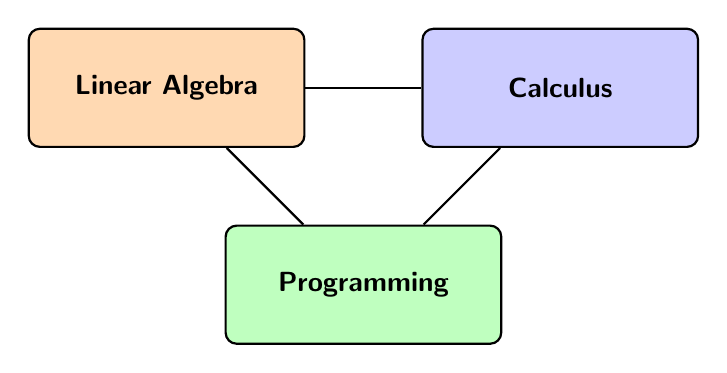
\begin{tikzpicture}[
    every node/.style={
        font=\sffamily\bfseries,
        minimum height=1.5cm,
        minimum width=3.5cm,
        align=center,
        rounded corners,
        draw=black,
        thick
    },
    arrow/.style={->, thick, >=Stealth, line width=1mm},
]

% Colored nodes
\node[fill=orange!30] (linAlg) at (0, 2.5) {Linear Algebra};
\node[fill=blue!20]   (calc)   at (5, 2.5) {Calculus};
\node[fill=green!25]  (prog)   at (2.5, 0) {Programming};

% Arrows (triangle)
\draw[thick] (linAlg) -- (calc);
\draw[thick] (calc) -- (prog);
\draw[thick] (prog) -- (linAlg);

\end{tikzpicture}

\end{frame}



% -------------------------------------------------
\begin{frame}{Some Algorithms you will Learn}

\begin{block}{Derivatives} 
\begin{itemize}
  \item Forward Difference
  \item Central Difference
  \item Richardson Extrapolation
\end{itemize}
\end{block}

\begin{block}{Integrals} 
\begin{itemize}
  \item Riemann Sum 
  \item Trapezoidal Rule
  \item Gaussian Quadrature
\end{itemize}
\end{block}

\begin{block}{Linear Algebra} 
\begin{itemize}
\item Gaussian Elimination
  \item LU Decomposition
  \item Power Method
\end{itemize}
\end{block}
\end{frame}

% -------------------------------------------------
\begin{frame}{Numerical vs.~Symbolic Computation}
This course is on \textbf{Numerical Computation}, not \textbf{Symbolic Computation}
\begin{block}{Numerical Computation}
    \begin{itemize}
        \item Operate on numbers to get a numerical result
        \item Example: 
        \[
        \frac{(17.36)^2 - 1}{17.36 + 1} = 16.36
        \]
    \end{itemize}
\end{block}

\begin{block}{Symbolic Computation}
    \begin{itemize}
        \item Operate on symbols to get an expression
        \item Example: 
        \[
        \frac{x^2 - 1}{x + 1} = x-1
        \]
    \end{itemize}
\end{block}

\end{frame}
% -------------------------------------------------
% -------------------------------------------------
\begin{frame}
\frametitle{Analytic vs.~Numerical Solution}

\textbf{Problem}: What number $x$ satisfies:  $$e^x = 3\pi $$
\begin{block}{Analytical Solution}
\begin{itemize}
    \item The exact numerical or symbolic representation of the solution.
    \item May use special characters such as $\pi$, $e$, or even variables
    \item Analytical Solution:
    $$ x = \ln(3\pi)$$
\end{itemize}

\end{block}
\begin{block}{Numerical Solution}
\begin{itemize}
    \item Numerical Solution: The computational representation of the solution
    \item Entirely numerical. It is usually an approximation.
    \item Numerical Solution:
    $$ x \approx 2.24334217$$
\end{itemize}
\end{block}

\end{frame}
% -------------------------------------------------
% \begin{frame}
% \frametitle{Numerical Computation and Approximation}
% \begin{itemize}
% \item Numerical Approximation is needed to carry out the steps in the
% numerical calculation.  The overall process is a numerical computation.
% \begin{example}[symbolic computation, numerical solution]
% \[
% \frac{1}{2} +
% \frac{1}{3} +
% \frac{1}{4} - 1 = \frac{1}{12} = 0.083333333\dots
% \]
% \end{example}
% \begin{example}[numerical computation, numerical approximation]
% \[
% 0.500 +
% 0.333 +
% 0.250
% - 1.000 = 0.083
% \]
% \end{example}
% \end{itemize}
% \end{frame}
% -------------------------------------------------
\begin{frame}{Levels of Abstraction}

\begin{block}{Method}
    A \textbf{method} is a general framework describing the solution process.
\end{block}
\begin{block}{Algorithm}
    An \textbf{algorithm} is a detailed description of executing the method. Think of psuedocode. 
\end{block}

\begin{block}{Implementation}
    An \textbf{implementation} is a particular instantiation of an algorithm. Think of software.  
\end{block}
\begin{center}
    divide-and-conquer sort $\rightarrow$ heap sort $\rightarrow$ the acutal code
\end{center}

\end{frame}
% -------------------------------------------------
% -------------------------------------------------
\begin{frame}{Major Theme}
\begin{columns}
\begin{column}{0.45\textwidth}
\pgfimage[height=4cm]{./figs/pull1}

\begin{center}
  \begin{block}{}
    Accuracy
  \end{block}
\end{center}
\end{column}

\begin{column}{0.45\textwidth}
\pgfimage[height=4cm]{./figs/pull2}

\begin{center}
  \begin{block}{}
    Cost
  \end{block}
\end{center}
\end{column}
\end{columns}
\begin{itemize}
    \item There is no ``best" algorithm
    \item You must to sacrifice accuracy for speed, and vice versa
\end{itemize}
\end{frame}
% -------------------------------------------------
\sectionframe{History of Pi}
% -------------------------------------------------
\begin{frame}{Ancient Egypt}
\begin{itemize}
\item 1650 BC: The Rhind Papyrus of ancient Egypt contains 85
problems; many use numerical algorithms (T. Chartier, Davidson)
\end{itemize}
\begin{columns}
  \begin{column}{0.55\textwidth}
    \pgfimage[height=6cm]{./figs/rhind}
  \end{column}
  \begin{column}{0.35\textwidth}
    \begin{itemize}
        \item Approximates $\pi$ with $(8/9)^2 * 4 \approx 3.1605$\\[5mm]

        \item More of a formula than an algorithm
    \end{itemize}
  \end{column}
\end{columns}
\end{frame}
% -------------------------------------------------
% -------------------------------------------------
\begin{frame}{Archimedes - Ancient Greece}
\begin{columns}
  \begin{column}{0.55\textwidth}
    \begin{itemize}
    \item 287-212BC - ``\textbf{Method of Exhaustion}"
    \item Method for determining $\pi$
      \begin{itemize}
        \item draw an $n$-sided polygon inscribing the  circle 
        \item draw an $n$-sided polygon circumscribing the circle 
        \item estimate the circumference
        \item calculate pi: $\pi \approx C/D$
      \end{itemize}
    \item Two digits of precision
    \end{itemize}
  \end{column}
  \begin{column}{0.35\textwidth}
    \pgfimage[height=4cm]{./figs/archimedes}
  \end{column}
\end{columns}
\end{frame}
\begin{frame}{Importance: Method of Exhaustion}


\begin{itemize}
  \item $C_n$ = circumference of an n-sided polygon 
  \item $\lim_{n\rightarrow\infty} C_n = \pi$
\end{itemize}
\begin{figure}
    \centering
    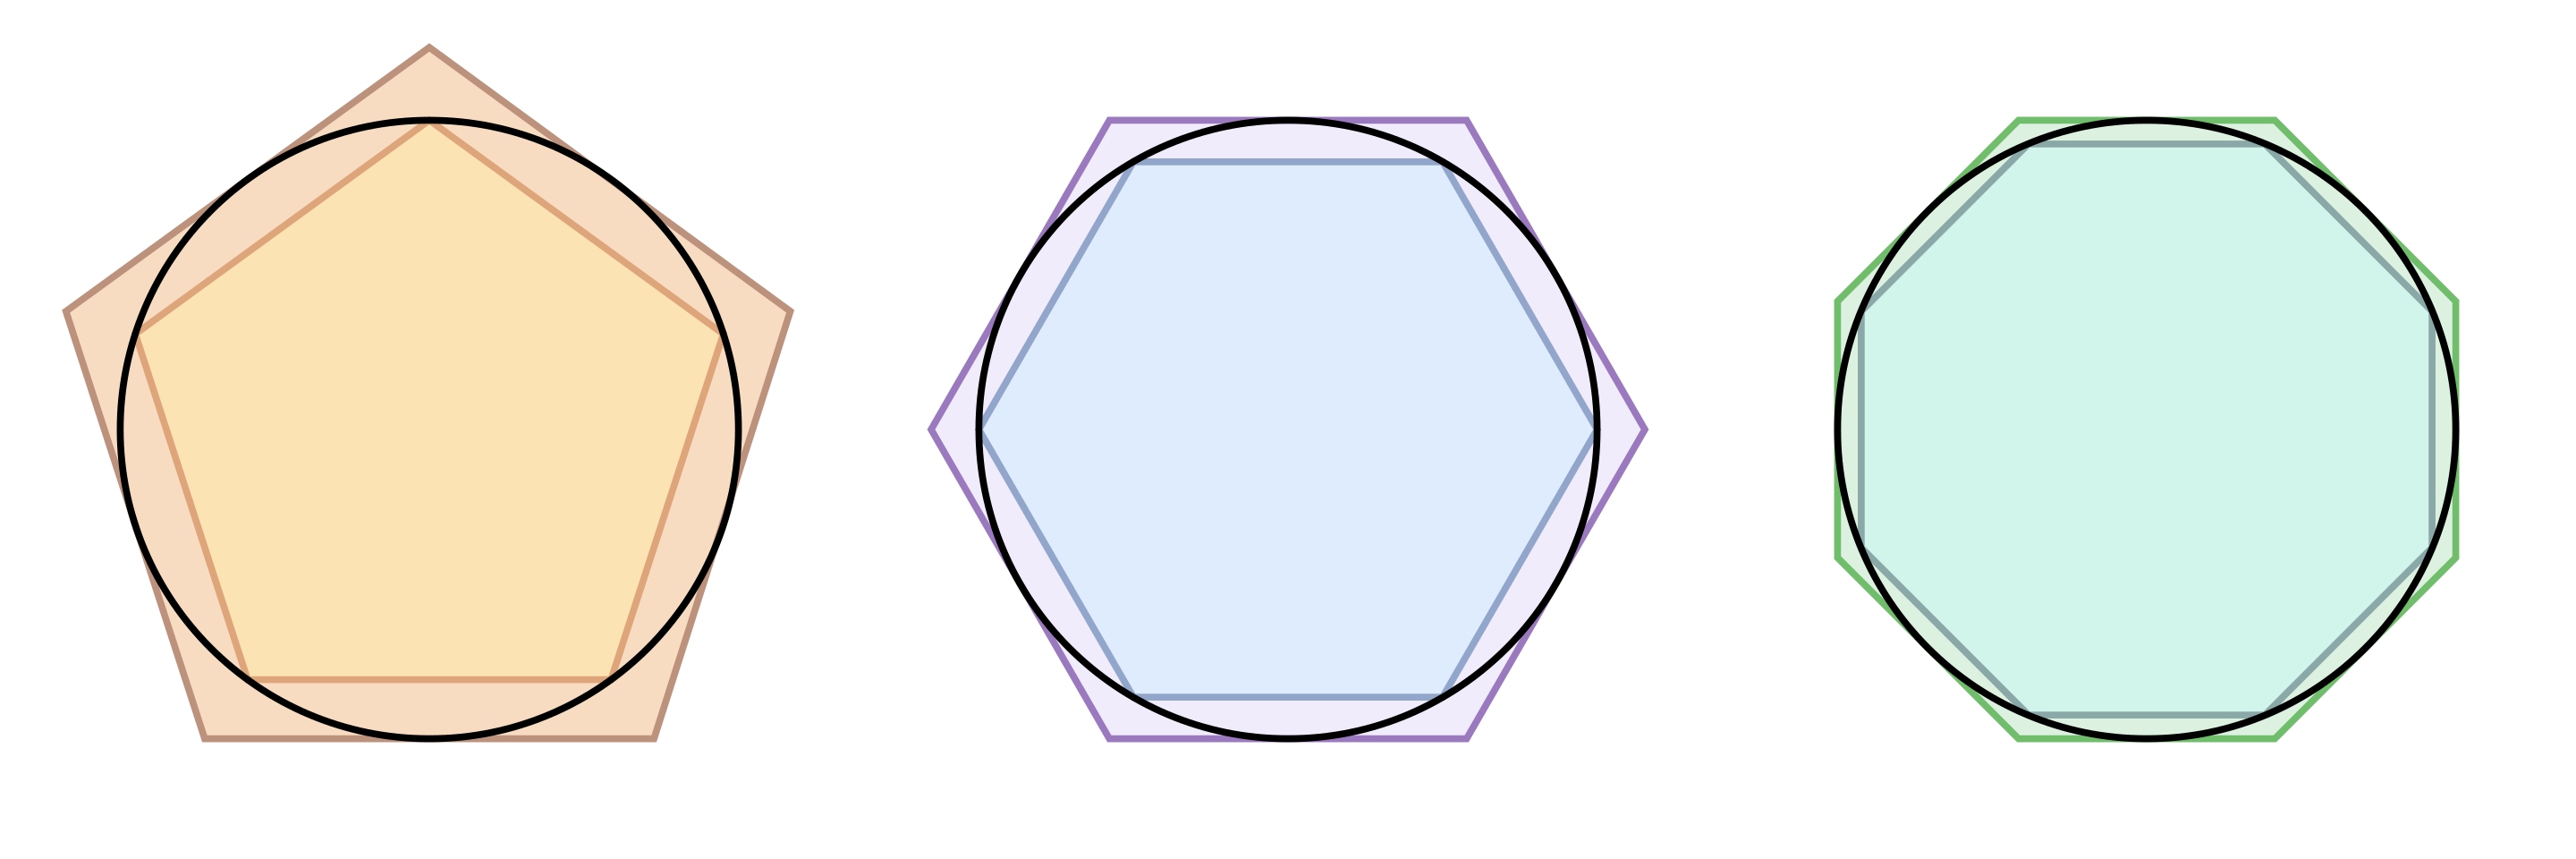
\includegraphics[width=0.7\linewidth]{figs/exhaution.png}
\end{figure}


\keyidea{
    \begin{itemize} 
        \item The number $n$ is a \underline{parameter} for the algorithm.
        \item As $n$ grows, algorithm gets \textbf{more expensive} but also \textbf{more accurate}.
    \end{itemize}
}

\end{frame}
% -------------------------------------------------
% -------------------------------------------------
\begin{frame}{Modern}
\begin{itemize}
  \item 1700s - John Machin discovered used identity to calculate 100 digits
  \begin{equation*}
  \pi  = 16 \arctan{(\frac{1}{5})} - 4\arctan{(\frac{1}{239})}
  \end{equation*}
\end{itemize}

  \begin{columns}
  \begin{column}{0.25\textwidth}
    
\includegraphics[scale=0.1]{figs/pi.jpg}
  \end{column}
  \begin{column}{0.55\textwidth}
    \begin{itemize}
        \item 1970s - $\pi$ computed to million digits using \textbf{Taylor series}
          \begin{equation*}
            \arctan{(x)} = x - \frac{x^3}{3} + \frac{x^5}{5} - \frac{x^7}{7}\dots
          \end{equation*}
        \item Let computers do all of the leg work
    \end{itemize}
  \end{column}
\end{columns}
\end{frame}


% -------------------------------------------------
\sectionframe{Why Study Computing?}
% -------------------------------------------------

\begin{frame}{Career in Computing}
\begin{block}{Scientific Computing}
\begin{itemize}
    \item \textbf{Scientific Computing} is a field where real-world problems are simplified to mathematical models and solved using computational algorithms.
    \item Must know math and programming
    \item Must also know the context: physics, biology, statistics, etc.
\end{itemize}
\end{block}
\bigskip
Scientists enable \textbf{simulation} which plays a vital role in the development of technology
\begin{itemize}
\item Safety
\item Optimization 
\item Analysis 
\end{itemize}
\end{frame}
% --------------------------------------------------
\begin{frame}{Applications}
Data produced by computational scientists:
\pgfimage[height=6cm]{./figs/eng_apps}
\begin{center}
Numerical computing is vital in engineering
\end{center}
\end{frame}

% -------------------------------------------------

\begin{frame}{More Applications}
Outside of engineering:
\begin{itemize}
    \item \textbf{AI}:  transitions, state systems, patterns (eigenvalues, linear algebra)
    \item \textbf{Informatics}:  Google matrix, Amazon recommendations (eigenvalues, linear
    algebra, sparse matrices, iterative methods)
    \item \textbf{Graphics}:  image compression, representation of
    curves/surfaces/lighting (interpolation, differentiation, etc)
    \item \textbf{Security}:  ssh (random numbers)
    \item \textbf{Economics/Finance}:  modeling/simulation of financial data (monte carlo)
    \item \textbf{High performance computing}: design of algorithms for rapid/parallel computing.
    \end{itemize}
\end{frame}

% -------------------------------------------------
\sectionframe{Analysis of Algorithms}
% -------------------------------------------------
\begin{frame}
\frametitle{Numerical Analysis}
\begin{block}{Numerical Analysis}    
\textbf{Numerical analysis} is the study of algorithms for the problems of continuous mathematics. 
\end{block}

\bigskip
\question{

\begin{itemize}
\item How do these algorithms work and how do they fail? (math theory)
\item To what degree can we trust these algorithms? (error analysis)
\item How expensive are these algorithms and will it scale well? (algorithmic efficiency)
\end{itemize}
}

\end{frame}


% -------------------------------------------------
\begin{frame}{The Big Three}

For any algorithm we study, we want to know: \bigskip

\begin{description}
\item[Accuracy] How accurate is the approximated solution? How reliable are the algorithmic outputs?\\  \bigskip

\item[Efficiency] How fast and cheap (in terms of operations and memory) can we compute a solution with respect to problem size?\\ \bigskip

\item[Stability] Is the computed solution sensitive to changes in the problem parameters? If there's a small offset in the in the conditions, will I get a completely different answer? 
\end{description}
\end{frame}

% --------------------------------------------------
\begin{frame}{Analysis is Important!}
Some disasters attributable to bad numerical computing:\\[6mm]

\begin{itemize}
\item The Patriot Missile failure, in Dharan, Saudi Arabia, on February 25, 1991 which resulted in 28 deaths, is ultimately attributable to poor handling of \underline{rounding errors}.\\[3mm]

\item The explosion of the Ariane 5 rocket just after lift-off on its maiden voyage off French Guiana, on June 4, 1996, was ultimately the consequence of a simple \underline{overflow}.\\[3mm]

\item The sinking of the Sleipner A offshore platform in Gandsfjorden near Stavanger, Norway, on August 23, 1991, resulted in a loss of nearly one billion dollars. It was found to be the result of a \underline{discretization model} of the finite element system.\\[3mm]

\end{itemize}

\end{frame}


% -------------------------------------------------
% -------------------------------------------------
% \begin{frame}
% \frametitle{Course Info}

% Basic Course Info:
% \begin{itemize}
%    \item Class Meetings: \newline
%       Tues at 11am-12:15pm, Face-to-Face, Mitchell 220 \newline
%       Thurs at 11am-12:15pm, Virtually (Link available on UNM Learn)
%       \smallskip
%       \smallskip
%    %\item Jacob's Office: SMLC 332
%    \item Zoom Drop-In Hours (link available on UNM Learn): 
%       \newline Wednesday 11:00am-12:30pm 
%       \newline Thursday 9:00am-10:30am
      
%       \smallskip
%       \smallskip
%    \item Email: jbschroder@unm.edu
% \end{itemize}

% \begin{columns}
% \begin{column}{0.8\textwidth}
% \begin{itemize}
% \item Thursday's virtual class will be remote synchronous and will function like a normal lecture.  \newline
%  $\Rightarrow$ I will make every effort to record these lectures and post the videos (please remind me if you don't see the record icon on Thursdays).
% \smallskip
% \smallskip
% \item Book:\newline
%    Numerical Mathematics and Computing, Seventh Edition, by Cheney and Kincaid (or 6th)%\newline
%    %\textbf{OR} \newline
%    %Numerical Analysis by T. Sauer, 3rd Edition\vspace{3pt} \newline  
%    %\textit{\small You will need one of these books as a reference, to buttress the
%    %   in-course slides and derivations. Sauer is likely a better general
%    %   reference book, but some course material will more closely follow Cheney
%    %   and Kincaid.}
% \end{itemize}
% \end{column}
% \begin{column}{\textwidth}
% \pgfimage[height=3cm]{./figs/nmc}
% \end{column}
% \end{columns}

% \bigskip
% {\small

% }
% \end{frame}

% -------------------------------------------------
\sectionframe{Course Info}
% -------------------------------------------------
\begin{frame}{Course Info}
All information about the course can be found on the syllabus or Canvas home page
\begin{block}{Topics}
   \begin{itemize}
      \item All class meetings and Drop-in Hours
      \item HW Policy
      % \item COVID Policy
      \item Dates Dates
      \item Grading rubric
      \item Matlab tutorial
      \item Weekly schedule
      \item Online access to textbook
   \end{itemize}
%All course materials are at  \url{http://math.unm.edu/~schroder/2020_Spring_375/index.html}
\end{block}
\bigskip

\end{frame}
% -------------------------------------------------
% -------------------------------------------------


% -------------------------------------------------
% -------------------------------------------------
\begin{frame}{Assessment}

Grades:
\begin{tabular}{l l}
Homework       & 15\%\\
Midterms   & 60\%\\
Final     & 25\%\\
\end{tabular}
   \vspace{1em}

   Homework: 
\begin{itemize}
\item Weekly assignment/report
\item PDF must include: 
\begin{itemize}
    \item source code 
    \item output
    \item high-quality graphs
    \item answers to any questions  
\end{itemize}
\item 15\% penalty for each day late 
\item Lowest score dropped
\item Encouraged to work in groups of two
\end{itemize}
\end{frame}
% -------------------------------------------------
\begin{frame}{More Info}
\bigskip
Schedule and Notes:
\begin{itemize}
    \item Lecture involves slides + hand calculations 
    \item Attendance is mandatory
    \item Final exam is fixed
       \bigskip
   \item You may ask for accommodations - HW extensions 
   \item Read the syllabus
   \item Course materials on Canvas
   \item Look at the MATLAB tutorial on website\newline
      $\Rightarrow$ \textbf{We will do the tutorial next class}
\end{itemize}


\bigskip
   
\end{frame}

\sectionframe{What to Expect}
% -------------------------------------------------
\begin{frame}{Typical Process}{1. Approach a problem using theory}
\begin{example}
  Find $f'(1.0)$ for function $f(x)=e^{x}$.\\
  (Assume you do not know the solution.)
\end{example}
\begin{block}{Theory}
The definition of the derivative
  \begin{equation*} 
    f'(x) := \lim_{h\rightarrow 0} \frac{f(x+h) - f(x)}{h}
    \end{equation*}
\end{block}
\begin{block}{Method}
Choose a small parameter $h>0$
  \begin{equation*} 
    f'(x) \approx \frac{f(x+h) - f(x)}{h}
\end{equation*}
\end{block}
\end{frame}
% -------------------------------------------------
% -------------------------------------------------
\begin{frame}[fragile]{Typical Process}{2. Design an algorithm and implement it}
\begin{block}{Implementation}
    Write out your algorithm by hand. Then write your method in Matlab.
\end{block}
\begin{columns}
\begin{column}{0.45\textwidth}
\begin{lstlisting}[mathescape,caption=Algorithm (by hand)]
$f(x) = e^x$
$x_0$=1  
$h = 10^{-2}$
$f'(x_0)\approx(f(x+h)- f(x))/h$ 
\end{lstlisting}
\end{column}

\begin{column}{0.45\textwidth}
\begin{lstlisting}[caption= Implementation (Matlab)]
f= @(x) (exp(x));
x0=1;
h=1e-2;
fp=(f(x+h) - f(x))/h;
\end{lstlisting}
\end{column}
\end{columns}

\vspace{3mm}
\begin{center}
    Translate the mathematical algorithm into code.
\end{center}
\end{frame}
% -------------------------------------------------
\begin{frame}{Typical Process}{3. Analyze the error}

    \begin{block}{Error Analysis}
        For this problem, we know the real answer, $f'(1.0) = e^{1.0} = e$. We can compute the error as a function of $h$. 
    \end{block}

 
    \begin{itemize}
    \item Method
  \begin{equation*} 
    f'(x) \approx \frac{f(x+h) - f(x)}{h}
    \end{equation*}

        \item Error 
        $$E(h) = \left| \underbrace{f'(x)}_{\text{true}} - \underbrace{\frac{f(x+h) - f(x)}{h}}_{\text{approximate}}\right|$$
    \end{itemize}

    \begin{block}{Be investigative}
    \begin{itemize}
        \item How quickly does the error decrease with respect to $h$?
        \item Does the convergence depend on $f(x)$?
    \end{itemize}
        
    \end{block}
\end{frame}

% -------------------------------------------------

\begin{frame}[shrink]{Colored Blocks in Lecture Slides}
    
{
\define{Terminology}{Definitions are in yellow blocks}
}

{
\method{Name of algorithm}{Algorithm inputs}{Algorithm output}{What makes the method special}
}

\begin{example}
Problem you may see on an exam
\end{example}

\keyidea{Important conceptual idea}

\question{Usually a segue question}

\end{frame}

\begin{frame}{What to Expect for Exams}

\textbf{Types of Questions:}
\begin{itemize}
    \item \textbf{Short calculations}  
    \begin{itemize}
        \item Example: Approximate $\sqrt{2}$ using a Taylor series
        \item Focus on setup and method, not long arithmetic
    \end{itemize}

    \item \textbf{Short answers}  
    \begin{itemize}
        \item Example: Explain why a method converges or fails
        \item Clear reasoning in words matters
    \end{itemize}

    \item \textbf{Derivations}  
    \begin{itemize}
        \item Reproduce key steps shown in lecture
        \item You will not be asked to invent proofs from scratch
    \end{itemize}

    \item \textbf{Graph and table interpretation}  
    \begin{itemize}
        \item Read plots, trends, stability, or behavior from visuals
    \end{itemize}

    \item \textbf{Concept checks}
    \begin{itemize}
        \item Multiple choice
        \item Fill-in-the-blank
        \item True/False 
    \end{itemize}
\end{itemize}
\begin{center}
    Use the review sheets to prepare for exams.
\end{center}
\end{frame}


\begin{frame}{Canvas}
    \begin{itemize}
        \item Schedule Page - One lecture slide per day 
        \begin{figure}
            \centering
            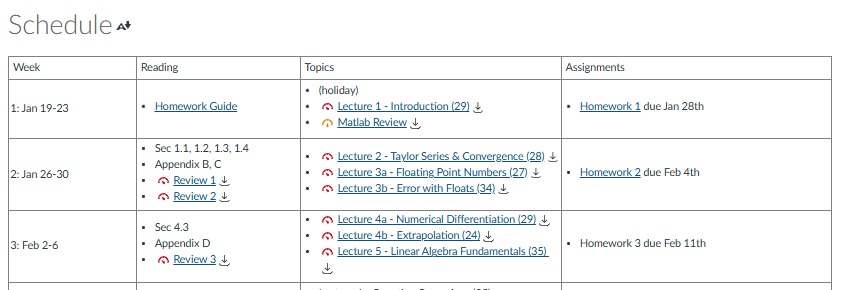
\includegraphics[width=0.9\linewidth]{figs/schedule.png}
        \end{figure}
        \item Modules - New module available every week
            \begin{figure}
            \centering
            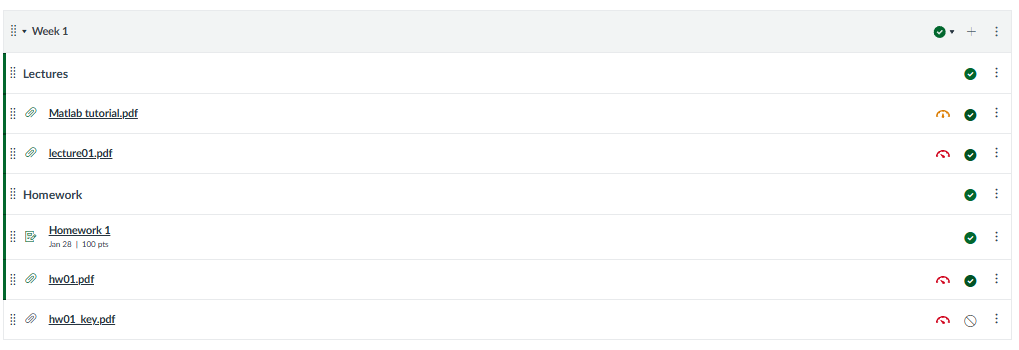
\includegraphics[width=0.9\linewidth]{figs/modules.png}
        \end{figure}
    \end{itemize}
\end{frame}


    
% -------------------------------------------------

\sectionframe{MATLAB}

% -------------------------------------------------
\begin{frame}
\frametitle{MATLAB}
\begin{itemize}
\item {\bf MAT}rix {\bf LAB}oratory
\item Both a computing environment and a language
\item Written in C. For matrix computations, it calls C/Fortran libraries == Fast
\item Matlab + ``Toolboxes''
  \begin{itemize}
  \item Symbolic Math Toolbox: mathematical manipulation of symbols
  \item Partial Differential Equation Toolbox: tools for solving PDEs in 2-D
  \item Statistics Toolbox: statistical data analysis
  \item Image processing toolbox: visualization and image analysis
  \item Bioinformatics toolbox: computational molecular biology
  \item Compiler: application development
  \item many many more.
  \end{itemize}
\item {\url{http://www.mathworks.com}}
\end{itemize}
\end{frame}
% -------------------------------------------------
\begin{frame}
\frametitle{MATLAB}
\begin{description}
    \item[The Good]  
        \begin{itemize}
        \item Beginner friendly
        \item No compiling
        \item Easy debugging $\rightarrow$ fast development
        \item Designed for linear algebra
        \item Great for plotting
        \item Great for generating reports
        \item Online editor + synced collaboration
        \end{itemize}
    \item[The Bad] 
        \begin{itemize}
        \item Computational overhead
        \item Very limited customization
        \end{itemize}
    \item[The Ugly]
        \begin{itemize}
        \item Proprietary and expensive (but free for UNM students)
        \item \sout{Can't update version???} Now you can
        \end{itemize}
\end{description}

\vspace{5mm}

\begin{center}
We will use Matlab for homework assignments. 
\end{center}
% $\Rightarrow$ \textbf{We will do the tutorial next class, have computer ready}
%Now, you can fire up Matlab and start the tutorial...
\end{frame}
% -------------------------------------------------

% \begin{frame}{Matlab Publish}
%     \begin{center}
%         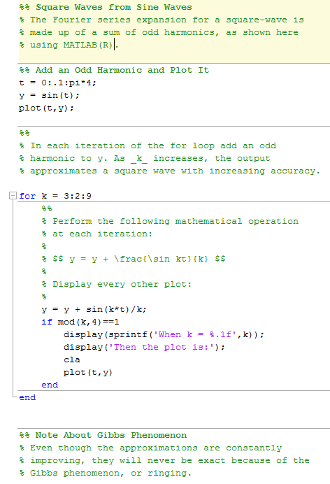
\includegraphics[scale=0.38]{figs/publish_code.png}\quad  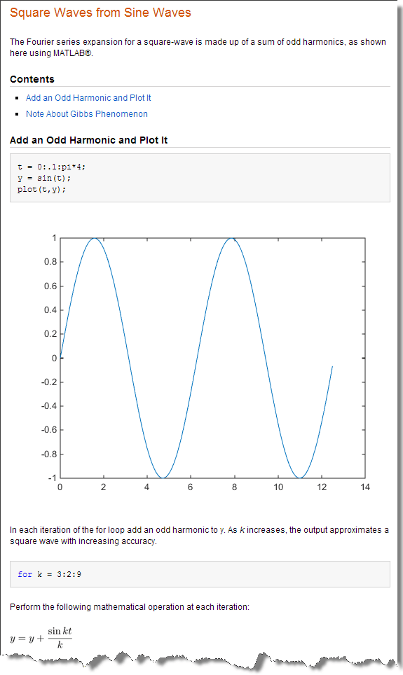
\includegraphics[scale=0.28]{figs/publish_output.png}
%     \end{center}
%     \begin{itemize}
%         \item Write Markup and LaTeX in the comments
%         \item Auto-generate a PDF with source code + output + text
%     \end{itemize}
% \end{frame}

% -------------------------------------------------

\begin{frame}{Matlab Live Script}
    \begin{center}
        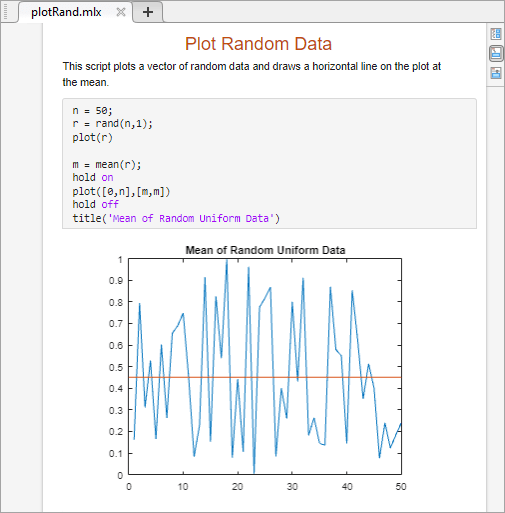
\includegraphics[scale=0.4]{figs/live_script.png}\
    \end{center}
    \begin{itemize}
        \item Combine code, output, and text all in one document
        \item Friendly UI
        \item Mathematical equations 
        \item Can include pictures 
        \item Easy to debug
    \end{itemize}
\end{frame}

\begin{frame}{Installation}
Matlab is covered by your tuition.\\
There are versions for Linux, Windows, and Mac. 

\bigskip 

\begin{enumerate}
    \item Go to \url{https://www.mathworks.com/}
    \item Click on Get MATLAB top right 
    \item Create an account with UNM email (or sign in)  
    \item Download and install latest version with your account 
\end{enumerate}

\bigskip 
\begin{block}{Matlab Online}
    You can also access Matlab on your browser at \url{matlab.mathworks.com}
\end{block}
\end{frame}

\begin{frame}{Todo List}
\begin{enumerate}
    \item Read the syllabus 
    \item Note the exam dates
    \item Skim through homework 1
    \item Read the homework tutorial 
    \item Create a Mathworks account
    \item (Optional) Find a partner for the homework 
\end{enumerate}
\end{frame}

%% \begin{frame}
%% \frametitle{What is Python?}
%% 
%% Full fledged, easy to use programming language\vspace{1em}
%% 
%% The Good:
%% \begin{itemize}
%% \item All the good stuff that Matlab has!
%% \item Large range of libraries
%% \item Free to use forever!
%% \item Language has full object oriented support
%% \item Jupyter notebooks are great for displaying text, code and figures in the same file
%% \end{itemize}
%% 
%% The Bad:
%% \begin{itemize}
%% \item Installing it and the associated libraries can be a pain (although many good installers now available)
%% \item Slightly steeper learning curve compared to Matlab
%% \end{itemize}
%% \end{frame}

% -------------------------------------------------
 \end{document}
